\documentclass[a4paper,11pt]{article} 
\usepackage{amsmath, amssymb, amsthm}
\usepackage{hyperref}
\usepackage{graphicx}
\usepackage{Sweave} %--------------------------------!
\newcommand{\pr}[2]{\underset{#1}{\mathbb{P}}\left[ #2 \right]}

\begin{document}
\Sconcordance{concordance:finalReport.tex:finalReport.Rnw:%
1 8 1 1 25 62 1 1 2 7 0 2 2 7 0 1 2 4 1 1 2 7 0 1 2 4 1 1 2 10 0 1 8 6 %
0 1 1 5 0 1 9 1 2 31 1 1 2 9 0 1 2 4 1 1 2 8 0 1 2 24 1 1 6 7 0 1 2 1 5 %
7 0 1 2 99 1 1 15 5 0 2 2 57 0 1 2 1 1 1 2 1 0 8 1 2 2 1 1 1 5 4 0 1 2 %
1 1 2 2 1 1 1 2 1 1 1 2 1 1 1 3 1 2 1 1 1 6 4 0 2 1 1 3 1 0 1 3 2 0 1 4 %
2 0 1 3 1 0 1 3 2 0 1 6 4 0 2 1 1 5 3 0 1 6 5 0 3 1 1 2 1 1 1 3 1 0 4 1 %
1 3 2 0 1 1 1 2 1 1 1 2 1 1 1 2 1 1 1 4 1 0 1 1 1 2 3 1 1 2 1 1 1 2 1 1 %
1 2 1 1 1 2 1 1 1 2 1 1 1 3 1 0 1 4 1 0 1 1 1 4 3 0 1 4 3 0 1 5 2 0 1 1 %
1 11 10 0 1 3 2 0 1 3 1 0 1 3 1 0 1 9 4 0 1 3 2 0 1 3 1 1 1 5 4 0 2 2 1 %
1 1 3 1 0 3 1 1 3 1 0 2 1 3 0 1 2 8 1}

\title{Prediction of Online News Popularity}
\author{G8}

\maketitle

\begin{section} 
{Introduction}
There is a \href{http://archive.ics.uci.edu/ml/datasets/Online+News+Popularity}{Dataset} provided in UCI Machine Learning Repository which summarizes a heterogeneous set of features about articles published by \href{http://mashable.com}{Mashable} in a period of two years. The goal is to predict the number of shares of these articles in social networks (popularity) [1]. The Dataset consists of 39,644 observations, with 61 variables. Each observation is related to an article published by Mashable in a period of two years. A short description of the articles' features is included in \textit{Appendix A}.\\
We are interested to study the popularity of articles and its relation to the proposed features, specially we want to figure out how these features contribute to the popularity of an article and what are the most significant ones or what are less important. Also we should mention that we are interested to investigate the popularity of those articles which their body have at least some text. The response variable which we want to predict is \textit{shares} as $Y$, and intuitively we have chosen 15 features which we think have the most effect on response variable. These selected features are listed in \textit{Appendix B}. Other features can be investigated if we encounter lack of fit.\\
To this end, we fit a multiple linear regression model to our data in order to be able to predict the number of shares of a given article based on our selected features and also make some inferences about the effect of these features on the popularity of an article.
\end{section}
%%%%%%%%%%%%%%%%%%%%%%%%%%%%%%%%%%%%%%%%%%%%%%%%%%%%%%%%%%%%%%%%%%%%%%%%%%%%%%%%%%
\begin{section}
{Methods}
\begin{subsection}{Initial Data Analysis}
The first thing we did was initial data analysis. We filtered our dataset in order to ensure the independence of observations assumption, clearly, if there is an article with reference to another article in the set, then the two corresponding observations are not independent, because one's number of shares will be affected by the other one's popularity. Hence, we have selected a subset of the observations which do not have any self-referenced articles. We also selected only those articles which contained at least some text in their body. This observation elimination, resulted in a dataset with \textbf{4169} observations which is still large enough for making statistical inferences. \\
The second step was looking into the distribution of our variables and find that if a transoformation in variables was appropriate. The response variable was highly positively skewed. The boxcox plot (\textit{Appendix C}) showed that a log transformation would be suitable. Also we have used $Sqrt$ transformation, for the number of images and number of vidoes features to reduce their intense skewness.\\
There was no missing value in the data. In terms of outliers, there are a few points which have a very large difference with other points in the dataset, but since the data is collected by means of computer programs, the probability that these points exist due to error in measurments is likely zero, hence it was not reasonable to omit these points at this stage of our study. We use a test for detecting outliers after we build our model.\\
In the third step, we looked for correlations between the variables. The correlation matrix, which is available in \textit{Appendix C}, shows that there is no significant correlation between our vriables of interest, except for $X_9$ and $X_{12}$, with 0.4, $X_3$ and $X_4$ with 0.3, and $X_{14}$ and $X_{15}$ with 0.3 pearson correlation.
\end{subsection}

\begin{subsection}{Feature Selection}
We divided our data into 3 parts, one with \textbf{2918} observations as the training set, one with \textbf{500} observations as the development set, and finally a set with \textbf{751} observations as the test set. Then we used exhaustive search to find the best explanatory features for the response variable. Two models were chosen according to two different criterions $adjR^2$ and $Bic$. The best model based on the proformance on development set was as follows:\\
$E\{ly\} = 7.2+0.023X_2-0.452X_3-0.063X_4+0.164X_5-0.016X_6-0.026X_7-0.329X_8-0.402X_{12}+0.487X_{13}+0.735X_{14}$.
\end{subsection}

\begin{subsection}{Model Assumptions}
We tested the selected model in order to validate the initial model assumptions by means of residual plots and ????.
\end{subsection}
\begin{subsection}{Bootstraping}
As the prvious results showed that the selected model assumptions cannot be validated, we used bootstrap in order to produce more reliable results. The use of bootstrap was meaningful, because we were sure about the independence of the observations.
\end{subsection}
\begin{subsection}{Performance Evaluation}
We used the provided test set in order to have an estimate of the performance of our model. We used $MSPR$ as a measure of performance for our linear regression model.
\end{subsection}
\end{section}
%%%%%%%%%%%%%%%%%%%%%%%%%%%%%%%%%%%%%%%%%%%%%%%%%%%%%%%%%%%%%%%%%%%%%%%%%%%%%%%%%%
\begin{section}{Results}
\begin{subsection}{Transformed variables}
The distributions of the variables after applying appropriate transformations for some of them are depicted in the figure \ref{dist-trans}.

\begin{figure}[h]
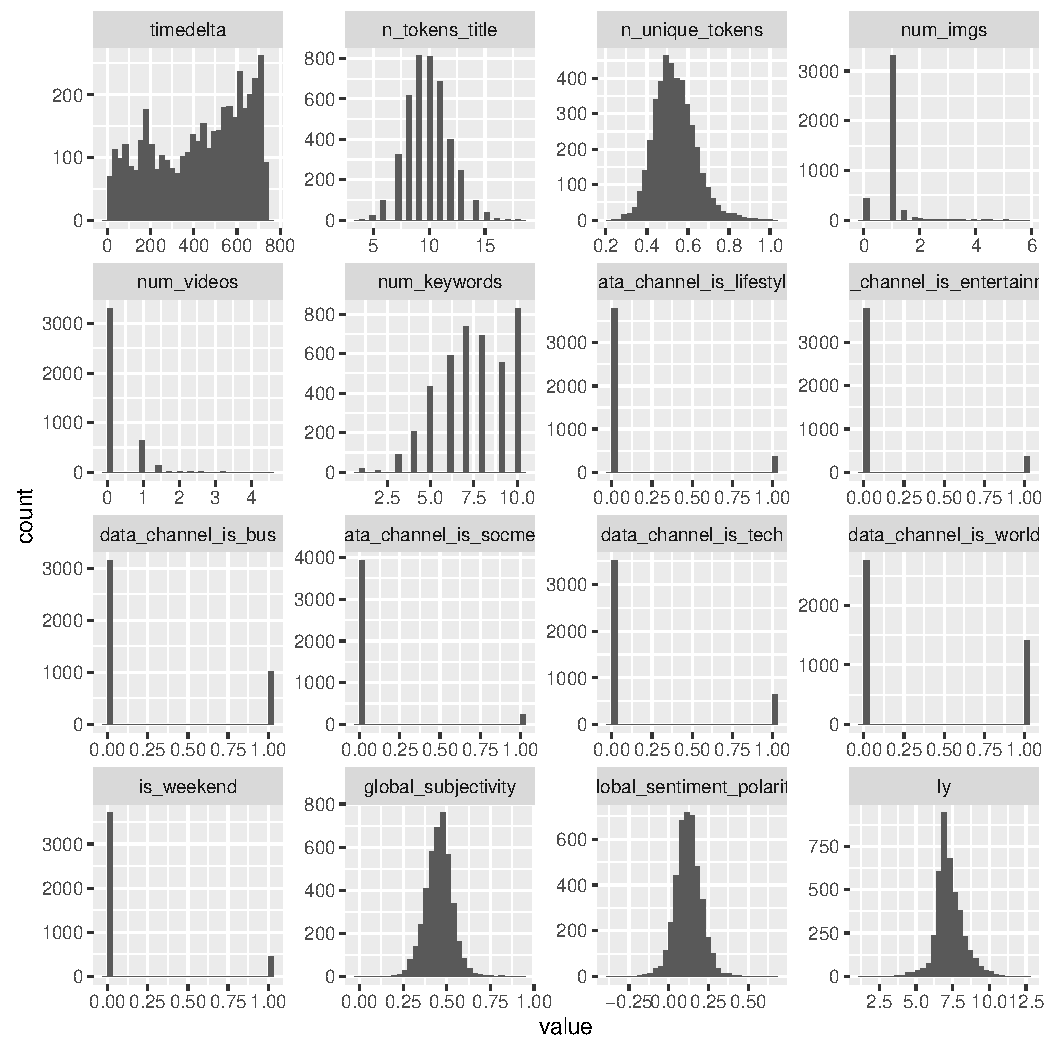
\includegraphics [width=7cm,height=7cm]{transformed-dists}
\centering
\caption{Distribbutions after Transformations}
\label{dist-trans}
\end{figure}

We see that the log transformation on response variable $ly$ was effective, and it made its distribution symetric and more similar to normal distribution. The $Sqrt$ transformation on $num_imgs$ and $num_videos$ was not able to reduce the skewness of the distributions, and that is because almost all of the articles have a few number of images and no videos.
\end{subsection}

\begin{subsection}{Selected Features}
Among the 15 features that we have, we used exhaustive search on different criterions like $RSS$, $CP$, $adjR^2$, and $Bic$ to select the best features. The result of this search is summarized in figure \ref{best-vis}.

\begin{figure}[h]
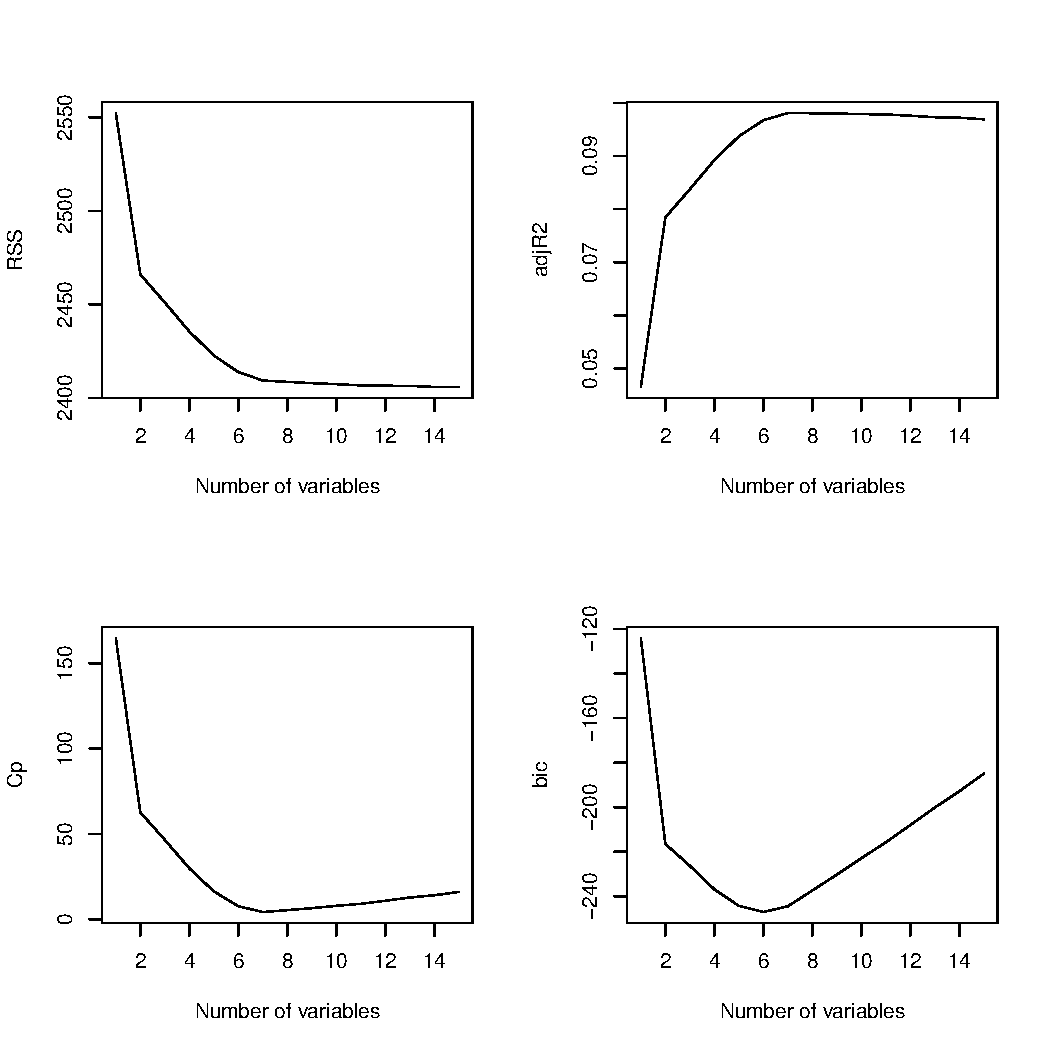
\includegraphics [width=7cm,height=7cm]{best-vis}
\centering
\caption{Best Model Visualization}
\label{best-vis}
\end{figure}

We see that the best model, would have around 6 to 9 predicators.\\
If we use $adjR^2$, $Cp$, or $RSS$ as our criteria of subset selection, then the best subset would be:
\begin{Schunk}
\begin{Soutput}
(Intercept)          X2          X3          X5          X6          X8 
 6.67550635  0.04289040 -0.23471826  0.15651311 -0.02389651 -0.46056053 
        X12         X13         X14 
-0.40774741  0.48304874  1.28578584 
\end{Soutput}
\end{Schunk}
and if we use $Bic$, then the best subset would be:
\begin{Schunk}
\begin{Soutput}
(Intercept)          X2          X5          X8         X12         X13 
 6.36426912  0.04420961  0.15550823 -0.46912422 -0.41000395  0.50204200 
        X14 
 1.27455978 
\end{Soutput}
\end{Schunk}
\end{subsection}

\begin{subsection}{Best Model Selection}
We have used the development set in order to choose between the first and the second model, which were introduced in the previous section. To this end, we use $MSPR$ as a metric for selecting the best model.\\
The $MSPR$s are:
\begin{Schunk}
\begin{Sinput}
>   c(mspr1,mspr2)
\end{Sinput}
\begin{Soutput}
[1] 0.8771907 0.8788786
\end{Soutput}
\end{Schunk}
Since $mspr1 < mspr2$, we choose the first model to investigate more.
\end{subsection}

\begin{subsection}{Removing Outliers}
The following test recognizes three of the data points as outliers, hence we remove these data points and rebuild our model again as previous.
\begin{Schunk}
\begin{Sinput}
> outlierTest(m1)
\end{Sinput}
\begin{Soutput}
      rstudent unadjusted p-value Bonferonni p
2593 -5.015317         5.6126e-07    0.0016378
1758  4.660357         3.2986e-06    0.0096254
1762  4.616032         4.0810e-06    0.0119080
\end{Soutput}
\end{Schunk}
\begin{Schunk}
\begin{Soutput}
(Intercept)          X2          X3          X5          X6          X8 
 6.67369174  0.04286074 -0.23555427  0.15730711 -0.02391254 -0.46364283 
        X12         X13         X14 
-0.40834625  0.48464918  1.29249182 
\end{Soutput}
\begin{Soutput}
(Intercept)          X2          X5          X8         X12         X13 
 6.36180657  0.04418551  0.15627445 -0.47245831 -0.41056064  0.50354302 
        X14 
 1.28127239 
\end{Soutput}
\end{Schunk}

After removing these point, the present variables in the previous model, are stll present and the performance on the development set increased just a little. however we contniue with the new model.
\end{subsection}

\begin{subsection}{Model Assumptions}
In this section we check if the linear regression model assumptions, can be verfied for our selected model in the previous part.
\begin{subsubsection}{Independence of observations}
As, we controlled the articles to have no reference to other articles in the set, and also as the article are chosen randomly from the available articles in Mashable, hence we can convince ourself that the observations are independent.
\end{subsubsection}

\begin{subsubsection}{Normality of residuals}
The QQ-plot for the residuals of our chosen model is as follows:\\

\begin{figure}[h]
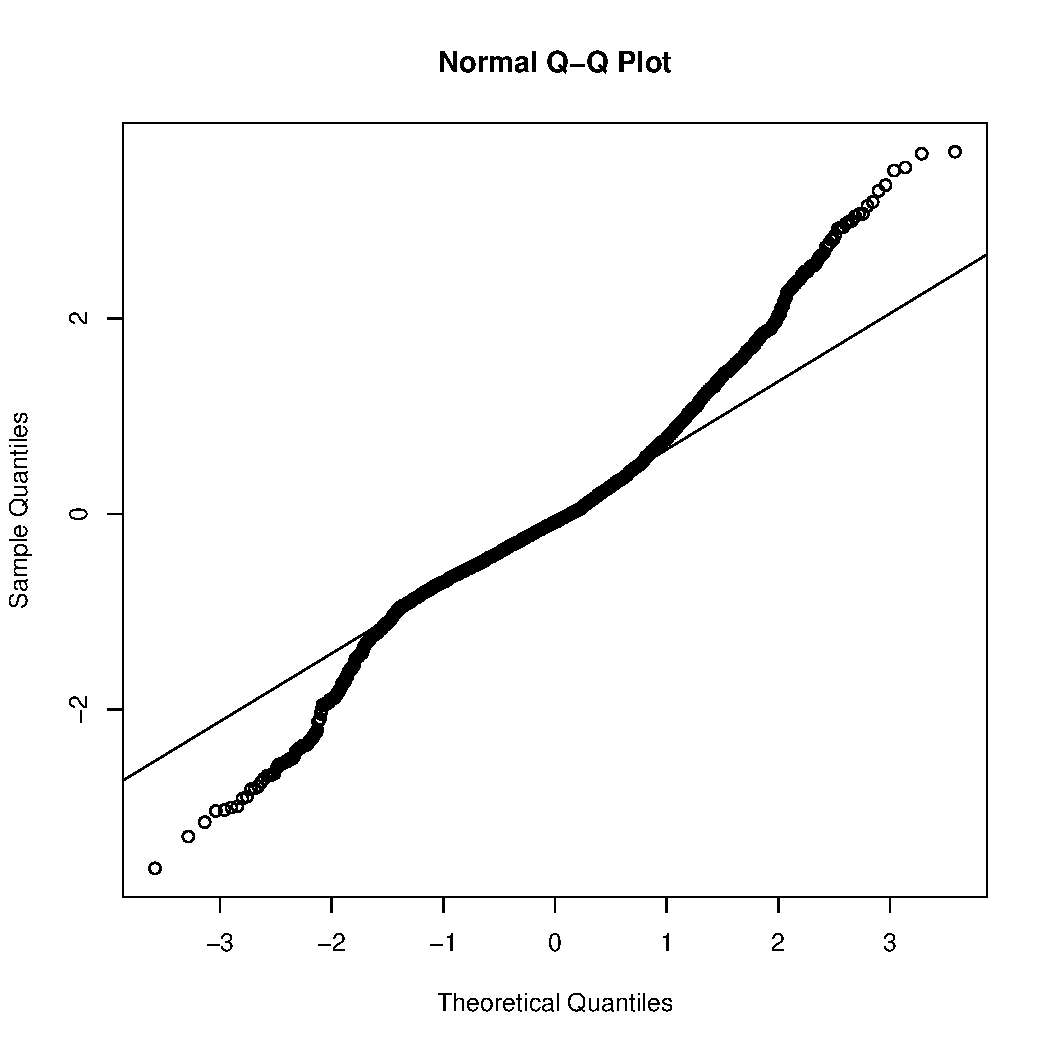
\includegraphics [width=3cm,height=3cm]{norm-ass}
\caption{QQ-plot of residuals}
\end{figure}

The deviation from normal distribution is obvious from this picture, hence we can conclude that the assumption of the normality of the eror terms was not adequate enough.
\end{subsubsection}
\begin{subsubsection}{Equal Variance}
The plot of absolute value of residuals versus the fitted values is:\\

\begin{figure}[h]
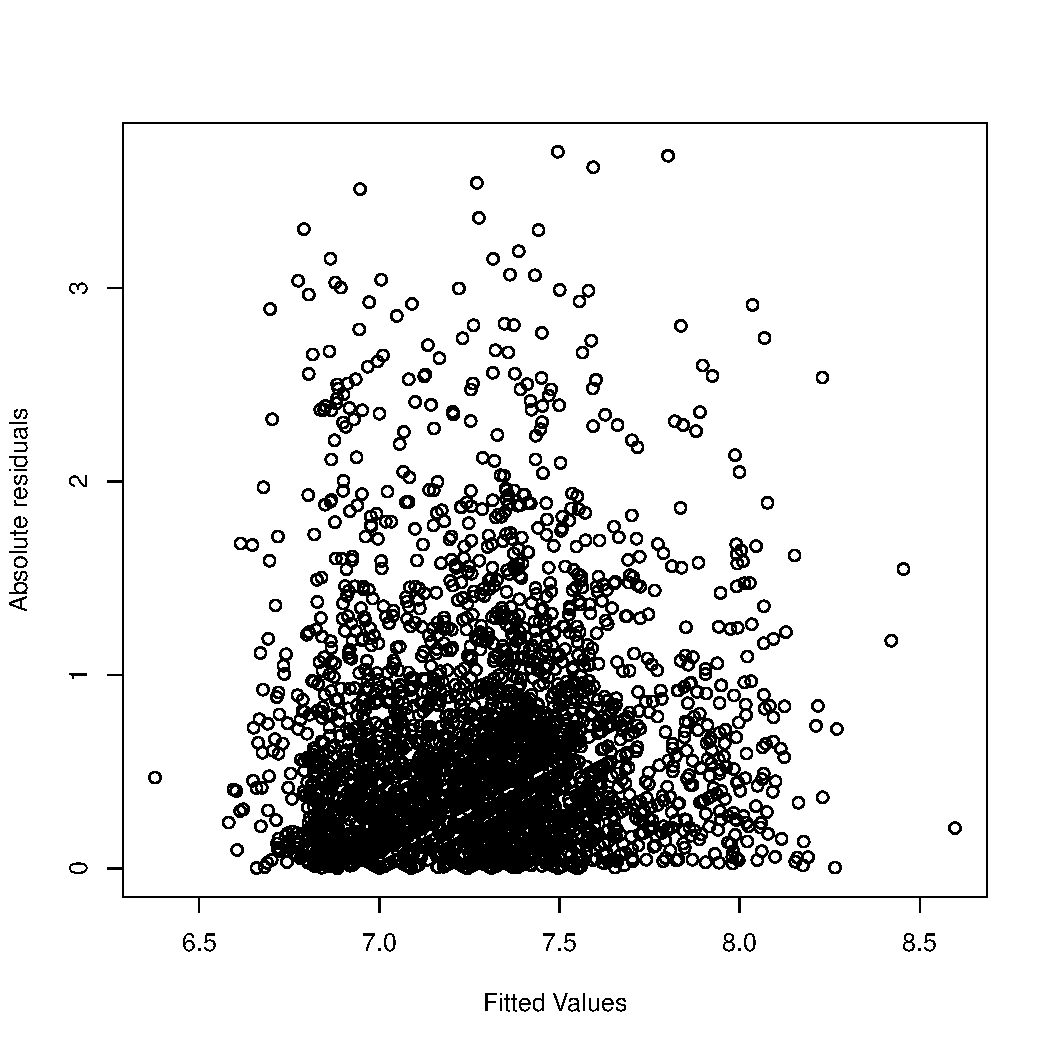
\includegraphics [width=4cm,height=4cm]{var-ass}
\caption{Absolute residuals vs Fitted values}
\label{var-ch}
\end{figure}

Figure \ref{var-ch}, shows that the assumption of equal variance was not well adequate. Because the spread of residuals changes several times when we have increase in the fitted values.

We also perform a Breusch-Pagan test to ensure that we are right about non-constant variance.
\begin{Schunk}
\begin{Sinput}
> ncvTest(m1_2)
\end{Sinput}
\begin{Soutput}
Non-constant Variance Score Test 
Variance formula: ~ fitted.values 
Chisquare = 3.752168    Df = 1     p = 0.05273906 
\end{Soutput}
\end{Schunk}
The high p-value above also shows that there is not enough evidence against the constant variance hypothesis.
\end{subsubsection}

\begin{subsubsection}{multicolinearity}
We compute variance inflation factors, in order to check if there is multicolinearity between our variables:
\begin{Schunk}
\begin{Sinput}
> vif(m1_2)
\end{Sinput}
\begin{Soutput}
      X2       X3       X5       X6       X8      X12      X13      X14 
1.019067 1.049346 1.054525 1.018702 1.090083 1.078718 1.021540 1.024043 
\end{Soutput}
\end{Schunk}
Since all the above values are very close to 1, we can conclude there is no multicolinearity among the variables in this model.
\end{subsubsection}

\begin{subsubsection}{Linear Relationship}
We use the residuals versus fitted values plot in order to check this assumption which is depicted in figure \ref{lin-rel}.

\begin{figure}[h]
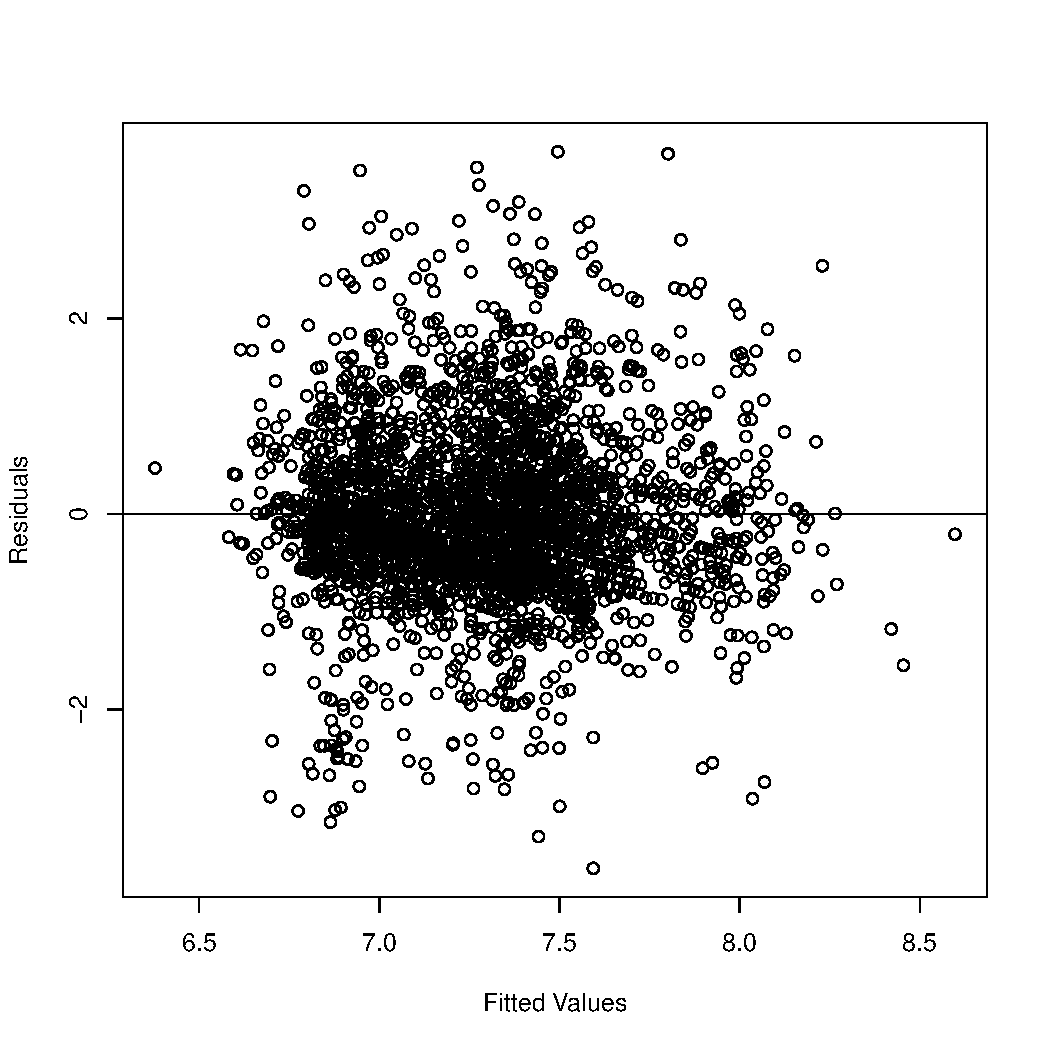
\includegraphics [width=4cm,height=4cm]{lin-rel}
\caption{Residuals vs Fitted values}
\label{lin-rel}
\end{figure}

As we cannot see any particular relation in the above plot, we can conclude that the assumption of linearity is adequate.
\end{subsubsection}

\end{subsection}


\begin{subsection}{Bootstrap}
As we have seen that the assumptions of normality and constant variance cannot be validated, we cannot make any statistical inference about the interplay between the features and response variables. Since the observations are independent, we use bootstrap technique to generate confidence intervals for the parameters in our previous regression model.\\
The 95\% confidence intervals for the parameters in our model would be as follows:\\
$\beta_0 \in (6.290, 7.063)$, $\beta_2 \in (0.0256, 0.0601)$, $\beta_3 \in (-0.6034, 0.1327)$, $\beta_5 \in ( 0.0837,  0.2259 )$, $\beta_6 \in  (-0.0402, -0.0066)$, $\beta_8 \in (-0.5801, -0.3382 )$, $\beta_{12} \in (-0.4732, -0.3396 )$, $\beta_{13} \in ( 0.3787,  0.5826 )$, $\beta_{14} \in ( 0.837,  1.718)$.
\end{subsection}
\begin{subsection}{Performance}
The performance of the linear model with best $Bic$ value, has the following $MSPR$ on the test set:
\begin{Schunk}
\begin{Sinput}
> mspr_ts
\end{Sinput}
\begin{Soutput}
[1] 0.8622303
\end{Soutput}
\end{Schunk}
And the linear model with averaged coefficients resulted from the bootstrap model, has the following $MSPR$:
\begin{Schunk}
\begin{Sinput}
> mspr_bt_ts
\end{Sinput}
\begin{Soutput}
[1] 0.86222
\end{Soutput}
\end{Schunk}
which shows that the bootstraped model performance has no significant difference from the previous model on the test set.
\end{subsection}
\end{section}
%####################################

\begin{section}{Discussion}
We have learned that there can be a linear association between the features and the response variable, but we cannot assume that error terms have normal distribution or have equal variances, which makes it impossible to fit a multiple linear regression model while all its assumptions are satisfied. We can use bootstrap to be confident enough about the strength of the effect of each variable on the response variable.\\
One interesting thing in this study was that $timedelta$ feature has no significant effect on the response variable, which means it is not important how long an article is published, its popularity is mostly determined by other factors. Also if the size of the content increases, then the popularity will decrease since we think that most people do not like to read long articles, But more informative titles (longer titles) have an inverse effect and causes an increase in the popularity.\\
The most effective features are $global_subjectivity$, and $is_weekend$ which shows that the articles which are published at weekends or contain stronger subjective texts are more likely to get popular.\\
In order to improve the result we can extend our study to also consider the omitted variables at the first step. We can also try other non-linear models to compare the results.

\end{section}

\begin{section}{References}
[1] K. Fernandes, P. Vinagre and P. Cortez. A Proactive Intelligent Decision
    Support System for Predicting the Popularity of Online News. Proceedings
    of the 17th EPIA 2015 - Portuguese Conference on Artificial Intelligence,
    September, Coimbra, Portugal.
\end{section}

\clearpage
\begin{section}{Appendix}
\textbf{Appendix A (short desciprion of the features)}\\
 Attribute Information:\\\\
     0. url:                    URL of the article\\
     1. timedelta:                  Days between the article publication and the dataset acquisition\\
     2. n\_tokens\_title:              Number of words in the title\\
     3. n\_tokens\_content:              Number of words in the content\\
     4. n\_unique\_tokens:               Rate of unique words in the content\\
     5. n\_non\_stop\_words:              Rate of non-stop words in the content\\
     6. n\_non\_stop\_unique\_tokens:      Rate of unique non-stop words in the content\\
     7. num\_hrefs:                     Number of links\\
     8. num\_self\_hrefs:                Number of links to other articles published by Mashable\\
     9. num\_imgs:                      Number of images\\
    10. num\_videos:                    Number of videos\\
    11. average\_token\_length:          Average length of the words in the content\\
    12. num\_keywords:                  Number of keywords in the metadata\\
    13. data\_channel\_is\_lifestyle:     Is data channel 'Lifestyle'?\\
    14. data\_channel\_is\_entertainment: Is data channel 'Entertainment'?\\
    15. data\_channel\_is\_bus:           Is data channel 'Business'?\\
    16. data\_channel\_is\_socmed:        Is data channel 'Social Media'?\\
    17. data\_channel\_is\_tech:          Is data channel 'Tech'?\\
    18. data\_channel\_is\_world:         Is data channel 'World'?\\
    19. kw\_min\_min:                    Worst keyword (min. shares)\\
    20. kw\_max\_min:                    Worst keyword (max. shares)\\
    21. kw\_avg\_min:                    Worst keyword (avg. shares)\\
    22. kw\_min\_max:                    Best keyword (min. shares)\\
    23. kw\_max\_max:                    Best keyword (max. shares)\\
    24. kw\_avg\_max:                    Best keyword (avg. shares)\\
    25. kw\_min\_avg:                    Avg. keyword (min. shares)\\
    26. kw\_max\_avg:                    Avg. keyword (max. shares)\\
    27. kw\_avg\_avg:                    Avg. keyword (avg. shares)\\
    28. self\_reference\_min\_shares:     Min. shares of referenced articles in
                                       Mashable\\
    29. self\_reference\_max\_shares:     Max. shares of referenced articles in
                                       Mashable\\
    30. self\_reference\_avg\_sharess:    Avg. shares of referenced articles in
                                       Mashable\\
    31. weekday\_is\_monday:             Was the article published on a Monday?\\
    32. weekday\_is\_tuesday:            Was the article published on a Tuesday?\\
    33. weekday\_is\_wednesday:          Was the article published on a Wednesday?\\
    34. weekday\_is\_thursday:           Was the article published on a Thursday?\\
    35. weekday\_is\_friday:             Was the article published on a Friday?\\
    36. weekday\_is\_saturday:           Was the article published on a Saturday?\\
    37. weekday\_is\_sunday:             Was the article published on a Sunday?\\
    38. is\_weekend:                    Was the article published on the weekend?\\
    39. LDA\_00:                        Closeness to LDA topic 0\\
    40. LDA\_01:                        Closeness to LDA topic 1\\
    41. LDA\_02:                        Closeness to LDA topic 2\\
    42. LDA\_03:                        Closeness to LDA topic 3\\
    43. LDA\_04:                        Closeness to LDA topic 4\\
    44. global\_subjectivity:           Text subjectivity\\
    45. global\_sentiment\_polarity:     Text sentiment polarity\\
    46. global\_rate\_positive\_words:    Rate of positive words in the content\\
    47. global\_rate\_negative\_words:    Rate of negative words in the content\\
    48. rate\_positive\_words:           Rate of positive words among non-neutral
                                       tokens\\
    49. rate\_negative\_words:           Rate of negative words among non-neutral
                                       tokens\\
    50. avg\_positive\_polarity:         Avg. polarity of positive words\\
    51. min\_positive\_polarity:         Min. polarity of positive words\\
    52. max\_positive\_polarity:         Max. polarity of positive words\\
    53. avg\_negative\_polarity:         Avg. polarity of negative  words\\
    54. min\_negative\_polarity:         Min. polarity of negative  words\\
    55. max\_negative\_polarity:         Max. polarity of negative  words\\
    56. title\_subjectivity:            Title subjectivity\\
    57. title\_sentiment\_polarity:      Title polarity\\
    58. abs\_title\_subjectivity:        Absolute subjectivity level\\
    59. abs\_title\_sentiment\_polarity:  Absolute polarity level\\
    60. shares:                        Number of shares (target)\\\\
   
   
\textbf{Appendix B (selected features):}\\\\
We have selected the following 15 features to study:\\
 $X_1: timedelta$,                     $X_2: n\_tokens\_title$,                $X_3: n\_unique\_tokens$,               $X_4: num\_imgs$,                     
  $X_5: num\_videos$\\                    $X_6: num\_keywords$\\                  $X_7: data\_channel\_is\_lifestyle$\\     $X_8: data\_channel\_is\_entertainment$\\
  $X_9: data\_channel\_is\_bus$\\           $X_{10}: data\_channel\_is\_socmed$\\        $X_{11}: data\_channel\_is\_tech$\\         $X_{12}: data\_channel\_is\_world$\\        
 $X_{13}: is\_weekend$\\                    $X_{14}: global\_subjectivity$\\           $X_{15}: global\_sentiment\_polarity$.\\\\

\textbf{Appendix C (transformation and correlations)}\\\\
\begin{Schunk}
\begin{Sinput}
> boxcox(y~.,data=dt)
\end{Sinput}
\end{Schunk}
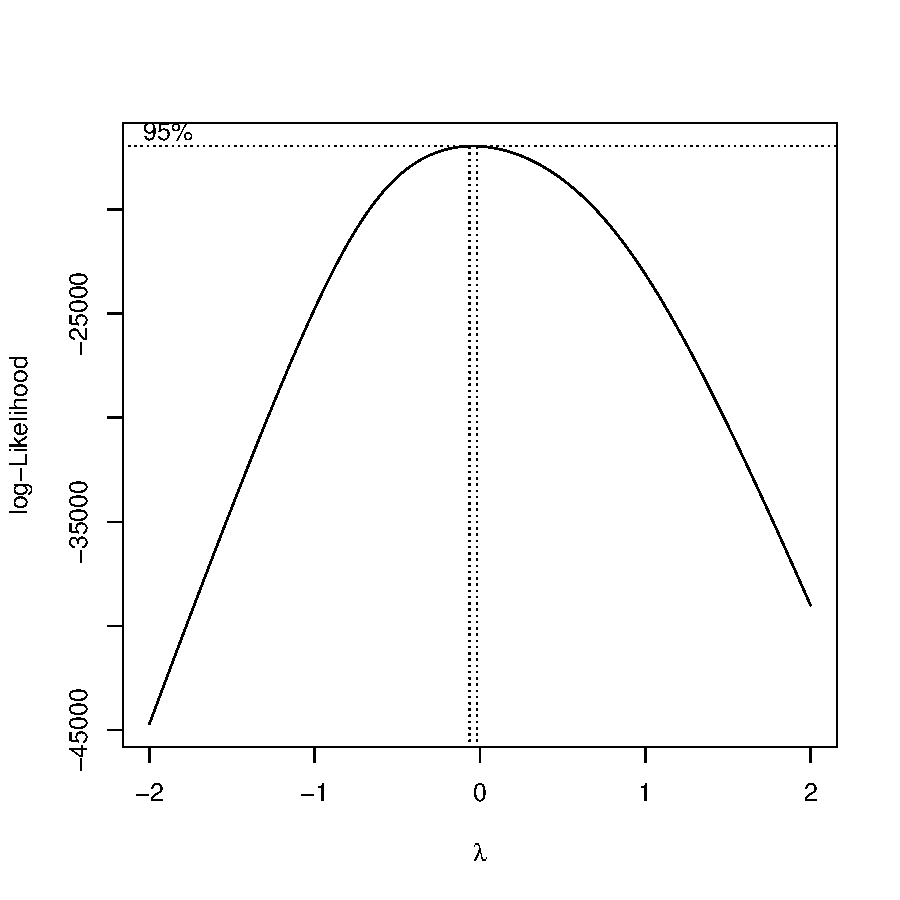
\includegraphics{finalReport-plot_plotboxcox}
And the correlation matrix between variables is:
\begin{Schunk}
\begin{Sinput}
> cor(dt)
\end{Sinput}
\begin{Soutput}
              X1          X2           X3           X4            X5
X1   1.000000000 -0.20561037  0.243430885 -0.164157698 -0.0415340908
X2  -0.205610365  1.00000000 -0.084711410  0.030211662  0.0280674386
X3   0.243430885 -0.08471141  1.000000000 -0.174499543  0.0912605923
X4  -0.164157698  0.03021166 -0.174499543  1.000000000 -0.0074471104
X5  -0.041534091  0.02806744  0.091260592 -0.007447110  1.0000000000
X6   0.162947215 -0.04242312 -0.038402341 -0.058453326 -0.0509553251
X7   0.034717960 -0.07886186 -0.010982241 -0.016805821  0.0005029448
X8   0.006837274  0.06476524  0.111020018  0.029184744  0.1096069167
X9   0.008847289  0.01716396 -0.116071484 -0.043537592 -0.0538937219
X10  0.051801215 -0.04802549 -0.002914681  0.012157183  0.0414117116
X11  0.124577511 -0.04549337  0.036357974 -0.010973229 -0.0619498323
X12 -0.192589446  0.05068610 -0.064030265  0.024757579 -0.0253661241
X13 -0.007539938  0.03173234 -0.053859625  0.014004296 -0.0175297449
X14  0.021084771 -0.02916178 -0.026758042 -0.018792627  0.0397494810
X15  0.053828178 -0.03127024 -0.018575581  0.001125627 -0.0053412252
y    0.042519849  0.03460153 -0.018433658 -0.012734525  0.0613121327
             X6            X7           X8           X9          X10
X1   0.16294722  0.0347179605  0.006837274  0.008847289  0.051801215
X2  -0.04242312 -0.0788618628  0.064765243  0.017163963 -0.048025492
X3  -0.03840234 -0.0109822408  0.111020018 -0.116071484 -0.002914681
X4  -0.05845333 -0.0168058213  0.029184744 -0.043537592  0.012157183
X5  -0.05095533  0.0005029448  0.109606917 -0.053893722  0.041411712
X6   1.00000000  0.0555167608 -0.014562611 -0.070452500 -0.160211338
X7   0.05551676  1.0000000000 -0.097674204 -0.175642797 -0.075307575
X8  -0.01456261 -0.0976742041  1.000000000 -0.178260642 -0.076429987
X9  -0.07045250 -0.1756427974 -0.178260642  1.000000000 -0.137440349
X10 -0.16021134 -0.0753075754 -0.076429987 -0.137440349  1.000000000
X11  0.13042790 -0.1325991539 -0.134575460 -0.242000542 -0.103758733
X12  0.02598162 -0.2217742331 -0.225079638 -0.404749827 -0.173538161
X13 -0.09318461 -0.0125355902 -0.009908673  0.051374531  0.023252024
X14  0.02888427  0.0769442751  0.063621971 -0.043429385  0.026867897
X15  0.03672954  0.0654776194 -0.008762452  0.208704014  0.015995154
y   -0.02007976  0.0381729473  0.017562773  0.017805385  0.033924272
            X11         X12          X13         X14          X15           y
X1   0.12457751 -0.19258945 -0.007539938  0.02108477  0.053828178  0.04251985
X2  -0.04549337  0.05068610  0.031732340 -0.02916178 -0.031270237  0.03460153
X3   0.03635797 -0.06403027 -0.053859625 -0.02675804 -0.018575581 -0.01843366
X4  -0.01097323  0.02475758  0.014004296 -0.01879263  0.001125627 -0.01273452
X5  -0.06194983 -0.02536612 -0.017529745  0.03974948 -0.005341225  0.06131213
X6   0.13042790  0.02598162 -0.093184614  0.02888427  0.036729544 -0.02007976
X7  -0.13259915 -0.22177423 -0.012535590  0.07694428  0.065477619  0.03817295
X8  -0.13457546 -0.22507964 -0.009908673  0.06362197 -0.008762452  0.01756277
X9  -0.24200054 -0.40474983  0.051374531 -0.04342938  0.208704014  0.01780538
X10 -0.10375873 -0.17353816  0.023252024  0.02686790  0.015995154  0.03392427
X11  1.00000000 -0.30556041  0.011394455  0.06676500  0.039693920  0.01724059
X12 -0.30556041  1.00000000 -0.058000959 -0.13634657 -0.271012321 -0.10072974
X13  0.01139445 -0.05800096  1.000000000  0.05016457  0.006713998  0.06054285
X14  0.06676500 -0.13634657  0.050164568  1.00000000  0.304312547  0.08945466
X15  0.03969392 -0.27101232  0.006713998  0.30431255  1.000000000  0.05124082
y    0.01724059 -0.10072974  0.060542849  0.08945466  0.051240817  1.00000000
\end{Soutput}
\end{Schunk}
\clearpage
\textbf{Appendix D (Code)}\\\\
\begin{Schunk}
\begin{Sinput}
> library(tidyr)
> library(dplyr)
> library(leaps)
> library(reshape2)
> library(ggplot2)
> library(Metrics)
> library(boot)
> library(car)
> library(MASS)
> setwd("/Users/Ehsan/Desktop/DataProj/")
> data_all <- read.csv("OnlineNewsPopularity.csv", stringsAsFactors = F)
> set.seed(123)
> data_filtered <- data_all %>%
+   filter(num_self_hrefs==0) %>%
+   filter(n_tokens_content != 0) %>%
+   arrange(timedelta) %>%
+   mutate(lshares=log(shares))
> data_selected <- data_filtered[,c(2,3,5,10,11,13:19,39,45:46, ncol(data_filtered)-1)]
> colnames(data_selected) <- c(paste("X",1:(ncol(data_selected)-1), sep=""),"y")
> boxcox(y~.,data=data_selected)
> qqnorm(data_selected$y)
> qqline(data_selected$y)
> y <- data_filtered$shares
> ly <- data_filtered$lshares
> qqnorm(ly)
> qqline(ly)
> x <- data_selected[,-ncol(data_selected)]
> boxplot(x[,4])
> boxplot(sqrt(x[,4]))
> #x1 : log
> #x4 : Sqrt
> #x5 : Sqrt
> 
> hist(x[,4])
> hist(sqrt(x[,5]))
> hist(log(sqrt(x[,4])))
> #pdf(file = "init-dists.pdf")
> d <- melt(cbind(x,y))
> ggplot(d,aes(x = value)) + 
+   facet_wrap(~variable,scales = "free") + 
+   geom_histogram()
> #dev.off()
> 
> x[,c(4,5)] <- sqrt(x[,c(4,5)])
> #pdf(file = "transformed-dists.pdf")
> d <- melt(cbind(x,ly))
> ggplot(d,aes(x = value)) + 
+   facet_wrap(~variable,scales = "free") + 
+   geom_histogram()
> #dev.off()
> 
> 
> 
> dt <- cbind(x,ly)
> names <- colnames(dt)
> colnames(dt) <- c(paste("X",1:ncol(x), sep=""),"ly")
> #write.csv(dt, "processedSet.csv", row.names = F)
> #dt <- read.csv("processedSet.csv", stringsAsFactors = F)
> 
> cor(dt)
> #X4 X3 0.3
> #X9 X12 -0.4
> #x14 X15 0.3
> 
> #--------------MODEL ASSUMPTIONS:
> tr <- sample_frac(dt, 0.7)
> tmp <- anti_join(dt,tr)
> dv <- sample_frac(tmp, 0.4)
> ts <- anti_join(tmp,dv)
> rg_exh <- regsubsets(ly~., tr,nvmax = 15)
> sm_exh <- summary(rg_exh)
> #pdf(file="best-vis.pdf")
> par(mfrow=c(2,2))
> plot(sm_exh$rss, xlab="Number of variables", ylab="RSS", type="l")
> plot(sm_exh$adjr2, xlab="Number of variables", ylab="adjR2", type="l")
> plot(sm_exh$cp, xlab="Number of variables", ylab="Cp", type="l")
> plot(sm_exh$bic, xlab="Number of variables", ylab="bic", type="l")
> #dev.off()
> 
> coef(rg_exh, which.max(sm_exh$adjr2))
> coef(rg_exh, which.min(sm_exh$bic))
> m1 <- lm(ly~X2+X3+X5+X6+X8+X12+X13+X14,tr)
> m2 <- lm(ly~X2+X5+X8+X12+X13+X14,tr)
> pr_m1 <- predict(m1,dv[,-ncol(dv)])
> pr_m2 <- predict(m2,dv[,-ncol(dv)])
> mspr1 <- rmse(pr_m1,dv[,ncol(dv)])^2
> mspr2 <- rmse(pr_m2,dv[,ncol(dv)])^2
> ##########Outliers
> outlierTest(m1)
> qqPlot(m1, main="QQ Plot")
> rem <- c(which(rownames(tr)==2593),which(rownames(tr)==1758),which(rownames(tr)==1762))
> tr2 <- tr[-rem,]
> rg_exh2 <- regsubsets(ly~., tr2,nvmax = 15)
> sm_exh2 <- summary(rg_exh)
> coef(rg_exh2, which.max(sm_exh2$adjr2))
> coef(rg_exh2, which.min(sm_exh2$bic))
> m1_2 <- lm(ly~X2+X3+X5+X6+X8+X12+X13+X14,tr2)
> m2_2 <- lm(ly~X2+X5+X8+X12+X13+X14,tr2)
> pr_m1_2 <- predict(m1_2,dv[,-ncol(dv)])
> pr_m2_2 <- predict(m2_2,dv[,-ncol(dv)])
> mspr1_2 <- rmse(pr_m1_2,dv[,ncol(dv)])^2
> mspr2_2 <- rmse(pr_m2_2,dv[,ncol(dv)])^2
> qqnorm(m1_2$residuals)
> qqline(m1_2$residuals)
> #Test for outliers again
> outlierTest(m1_2)
> #pdf(file = "norm-ass.pdf")
> qqnorm(m1_2$residuals)
> qqline(m1_2$residuals)
> #dev.off()
> 
> #pdf(file="var-ass.pdf")
> plot(y=abs(m1_2$residuals), x=m1_2$fitted.values, xlab="Fitted Values", ylab = "Absolute residuals")
> #dev.off()
> 
> #Test for variance
> ncvTest(m1_2)
> #test for linearity
> #pdf(file="lin-rel.pdf")
> plot(y=m1_2$residuals, x=m1_2$fitted.values, xlab="Fitted Values", ylab = "Residuals")
> abline(h=0)
> #dev.off()
> 
> #####################BOOT STRAP
> # I have 2918 obs. (population)
> # I choose samples of size 200 from this dataset.
> # 
> rsq <- function(formula, data, indices) {
+   d <- data[indices,] # allows boot to select sample 
+   fit <- lm(formula, data=d)
+   return(summary(fit)$adj.r.squared)
+ } 
> # bootstrapping with 1000 replications 
> adjr2 <- boot(data=tr, statistic=rsq, 
+                 R=1000, formula=ly~X2+X3+X5+X6+X8+X12+X13+X14)
> # view results
> plot(adjr2)
> # get 95% confidence interval 
> boot.ci(adjr2, type="norm")
> bs <- function(formula, data, indices) {
+   d <- data[indices,] # allows boot to select sample 
+   fit <- lm(formula, data=d)
+   return(coef(fit)) 
+ } 
> # bootstrapping with 1000 replications 
> coefs <- boot(data=tr, statistic=bs, 
+                 R=1000, formula=ly~X2+X3+X5+X6+X8+X12+X13+X14)
> bt_coefs <- apply(coefs$t,2,mean)
> bt_pr <- c()
> for(i in 1:nrow(ts)){
+   pr <- bt_coefs[1]+ts[i,"X2"]*bt_coefs[2]+ts[i,"X3"]*bt_coefs[3]+ts[i,"X5"]*bt_coefs[4]+ts[i,"X6"]*bt_coefs[5]+
+     ts[i,"X8"]*bt_coefs[6]+ts[i,"X12"]*bt_coefs[7]+ts[i,"X13"]*bt_coefs[8]+ts[i,"X14"]*bt_coefs[9]
+   bt_pr <- c(bt_pr,pr)
+ }
> mspr_bt <- rmse(bt_pr,ts[,ncol(ts)])^2
> pr_m1_2_ts <- predict(m1_2,ts[,-ncol(ts)])
> mspr_m_1_2_ts <- rmse(pr_m1_2_ts,ts[,ncol(ts)])^2
> # view results
> results
> plot(results, index=1) # intercept 
> plot(results, index=2) # X1
> plot(results, index=3) # X2 
> # get 95% confidence intervals 
> boot.ci(results, type="norm", index=1) # intercept 
> boot.ci(results, type="norm", index=2) # X1
> boot.ci(results, type="norm", index=3) # X2
\end{Sinput}
\end{Schunk}
\end{section}

\clearpage
\begin{section}{Statement of contributions}
All work is done by Ehsan RahimiNasab
\end{section}


\end{document}
